%% LyX 2.0.7 created this file.  For more info, see http://www.lyx.org/.
%% Do not edit unless you really know what you are doing.
\documentclass[english]{article}
\usepackage[T1]{fontenc}
\usepackage[latin9]{inputenc}
\usepackage{textcomp}
\usepackage{amstext}
\usepackage{graphicx}

\makeatletter

%%%%%%%%%%%%%%%%%%%%%%%%%%%%%% LyX specific LaTeX commands.
\newcommand{\lyxmathsym}[1]{\ifmmode\begingroup\def\b@ld{bold}
  \text{\ifx\math@version\b@ld\bfseries\fi#1}\endgroup\else#1\fi}

%% Because html converters don't know tabularnewline
\providecommand{\tabularnewline}{\\}
%% A simple dot to overcome graphicx limitations
\newcommand{\lyxdot}{.}


\@ifundefined{showcaptionsetup}{}{%
 \PassOptionsToPackage{caption=false}{subfig}}
\usepackage{subfig}
\makeatother

\usepackage{babel}
\begin{document}

\section{The data}

Additional to the media indicators, we collected the data base used
in drechselscheufle2011. This is large database comprising financial
indicators, surveys, prices and wages, indicators of the real economy,
and composite indicators. For details see Table \ref{tab:Indicators-and-labels}
in the appendix and drechselschheufle2011%
\footnote{Some variables are not included. We could not construct five spread
series involving corporate rates computed by Merryl Lynch and the
early bird indicator of the Commerzbank as we did not obtain the data.
Furthermore, we only obtained very short series for the purchasing
manager index of Markit. Finally, we did not include monetary aggregates
as there is no consistent concept of monetary aggregates for one country
since the introduction of the Euro in Germany.%
}. The different transformations of the raw data are either level (L),
differences (D), differences of natural logarithms (Dln) or second
differences of natural logarithms (D2ln). For the reference month
the data are available with a publication lag $k$ that varies from
0 to 2. 

However, unlike drechselscheufle2011 we employ real-time data, as
well. Revisions to measures of real economic activity such as employment,
sales, and in particular, industrial production are sometimes large,
and may occur years after official figures are first released. The
information set that has been available at different points in time,
the different vintages of the data, frequently convey a different
picture of the same period of time. Thus, the use of current-vintage
data, that is the data as they are available when the experiment is
implemented can lead an analyst to include variables in his forecasting
model that, in real time, have little marginal predictive power (see,
for example, orphanidesnorden2005 or koenigetal2003). Furthermore,
if we assume that revisions lead to an improvement of the indicators
this disadvantages indicators that are unrevised such as financial
data or the media data that are analysed here.


\section{Empirical set-up}

Due to the different release lags of indicators such as macroeconomic
or survey indicators, data unbalancedness often emerges at the end
of multivariate samples. This phenomenon is sometimes refered to as
the ragged-edge of the data. In order to account for this we adapt
the basic empirical set-up for individual models from DS2010 that
explicitly addresses this issue. The estimation equation for the individual
models is given as: 
\begin{equation}
Y_{t+h}^{h}=\alpha+\sum_{i=l}^{p}\beta_{i}Y_{t-i}+\sum_{j=k}^{q}\gamma_{j}X_{t-j}+\epsilon_{t+h}^{h}\label{eq:individual models}
\end{equation}


$Y_{t+h}^{h}$ is the annualized growth rate of industrial production
over the next $h$ month, $Y_{t+h}=1200/h\times\ln(IP_{t}/IP_{t-h})$.
The growth rate of industrial production in levels, $IP_{t}$, is
defined as $Y_{t}=\Delta\ln IP_{t}$. $X_{t}$ is a candidate predictor,
$\epsilon_{t+h}^{h}$ is an error term and $\alpha$, $\beta$, and
$\gamma$ are regression coefficients. The timely availability can
be taken account of by $l$ and $k$. German industrial production
is available only with a time lag of $l=3$ month. The publication
lag of the candidate regressors differ from $k=0$, mostly for financial
and media data, up to $k=2$ month. The lag length is optimized using
the Akaike information criterion. First, $p$ is estimated. Then,
holding $p$ fixed, $q$ is estimated.

Forecasts for 1 to 12 month horizons are computed in a pseudo-out-of-sample,
real-time set-up:
\begin{itemize}
\item The forecasts are based on the information set available to a forecaster
at the forecast origin, that is, the moment in time, the forecasts
are made. 
\item All real indicators are deflated using realtime CPI-data. 
\item The first forecast origin is 2005-12, the last one is 2014-11 for
h=1, respectively 2013:11 for h=12.
\item The estimations are based on a rolling window of 60 month. Employing
rolling windows increases adaptability to shocks see ??. Furthermore,
it is required for the MCS test (?auch white).
\item Each forecast origin, the lag-length are optimized and the model is
up-dated.
\end{itemize}

\section{Forecast evaluation}


\subsection{MSFE and Theil's U}

In the following, we concentrate on the standard loss function in
the forecasting literature, the squared forecast error, $L_{i,t}=e_{i,t}^{2}$.
Let $e_{i,t}=y_{t}-\widehat{y}_{i,t}$  be the forecast error of
model $i$  in period $t$, where $y_{t}$ is the realization of
the target variable and $\widehat{y}_{i,t}$ is the value forecasted
by model $i$. Usually, the forecast performance of alternative models
is compared using the mean squared forecast error (MSFE) defined as 

\begin{equation}
MSFE_{i}=\frac{\Sigma_{t=1}^{T}(e_{i,t})^{2}}{T},
\end{equation}
where $T$ is number of forecasts. However, by making use of squared
forecast errors the $MSFE_{i}$ tends to overly emphasize differences
between models. Thus, we will concentrate on the root mean squared
forecast error, $RMSFE_{i}$. For pairwise comparisons we employ the
Theil's U defined as
\begin{equation}
TU_{i}=\frac{RMSFE_{i}}{RMSFE_{0}}
\end{equation}


indicating the relative Performance of model $i$ with respect to
a benchmark model $i=0$. A positive value implies that the indicator
model is less accurate than the benchmark whereas a negative value
implies that it is more accurate than the benchmark. In line with
the literature our benchmark model is the autoregressive (AR) model.
It is defined as in Equation \ref{eq:individual models}, however,
there is no indicator variable included.


\subsection{Tests}


\subsubsection{Pairwise tests}

Our aim is it test if media data contain any valueable information
for forecasting purposes. A minimum requirement is that media data
improve forecasts from a simple autoregressive model. This involves
pairwise comparisons of the AR model and alternative models consisting
of the AR model augmented with an additional explanatory variables.
Let the loss difference be defined as $d_{i,t}=L_{0,t}-L_{i,t}$.
The starting point for pairwise forecast comparisons of a benchmark
model, $0$, and an alternative model $i$ is the DM1995 test statistic
defined as: 
\begin{equation}
DM=\frac{\overline{d_{i}}}{\widehat{V}(\overline{d_{i}})}
\end{equation}
 where $\overline{d}_{i}$ and $\widehat{V}(\overline{d_{i}})$ are
the estimated mean and long run variance of $d_{i,t}$, respectively.
The null hypothesis is

\begin{eqnarray}
H_{0}: & E[d_{i,t}]=0,\label{eq:dm null}
\end{eqnarray}
that is, that the two models perform equally good.

By construction, the AR is nested in the augmented model. Under the
null, the additional variables are useless and their coefficients
are zero. However, estimating additional variables introduces noise
into the forecasts of the alternative model. Consequently, under the
null the forecast accuracy of the smaller benchmark is higher than
for the larger alternative model, and not zero. Thus, in the context
of nested models, the DM statistic has lower power and size. Therefore,
we apply the modified test statistic of CW2007, CW-statistic that
involves an adjustment term to improve upon the DM-statistic when
nested models are compared:
\begin{equation}
CW=\frac{\overline{d_{i}}-\overline{a}_{i}}{\widehat{V}(\overline{d_{i}}-\overline{a}_{i})},
\end{equation}


where $\overline{a}_{i}=\frac{1}{T}\Sigma_{t=1}^{T}(\widehat{Y}_{0,t}-\widehat{Y}_{i,t})^{2}$.


\subsubsection{Multiple tests}

White2000 has pointed out, that even when no exploitable forecasting
relation exists, looking hard enough at a given set of data will often
reveal one or more forecasting models that look good, but are in fact
useless. Particulary, sequentially testing of a number of models two
at a time invalidates standard critical values and might result in
data snooping. In much of economic time series analysis this is aggrevated
by the fact that typically there is only a limited number of observations
available. To overcome this problem White2000, proposes a reality
check test, RC-test, for data snooping. He compares the whole set
of $m$ rival models at a time to the benchmark. The null hypothesis
is that none of the rival models is inferior to the benchmark

\begin{eqnarray}
H_{0}: & E[d_{i,t}]\leq0 & \forall i=1,...,m.\label{eq:white null}
\end{eqnarray}


It is rejected when at least one of the rivals yields significantly
better forecasts. the expected loss differential can be consistently
estimated using the sample mean $\overline{d}_{i}$. White proposes
the sample mean statistic
\begin{equation}
RC=\max_{k}P^{1/2}\overline{d}_{i}.
\end{equation}
This approach has subsequently been refined by Hansen2005. He shows
that the test statistic proposed by White is very conservative if
the set of rival models contains very poorly performing models and
proposes a refinement consisting of a studentized version of the WT-test
that is known as the test for superior predictive ability (SPA). 

However, selecting the benchmark independently of the data introduces
the problem of \textit{multiple comparisons} \textit{with control}.
To overcome this Hansen 2011 proposes the model confidence set, MCS;
which forms a set of best models, $\mathcal{M}*$, such that given
the set of all forecasting models, $\mathcal{M}_{0}$, the MCS identifies
the set of models that cannot be rejected as statistically inferior
at a certain level of confidence:

\begin{equation}
\mathcal{M}*=\left\{ i\in\mathcal{M}_{0}:\,\mu_{ij}\leq0\,\textrm{for}\,\textrm{all}\, j\in\mathcal{M}_{0}\right\} 
\end{equation}
where $\mu_{ij}=E(d_{ij})$ is the expected loss differential $d_{ij}=L_{it}-L_{jt}$
based on one-by-one comparisons of all models.%
\footnote{Here again, we choose the squared forecast error as loss.%
} The MCS is implemented using the following steps, where initially$\mathcal{M}$
is set $\mathcal{M}=\mathcal{M}_{0}$:
\begin{enumerate}
\item The null of equal predictive accuracy (EPA), $H_{0,\mathcal{M}}:\,\mu_{ij}\leq0\,\forall i,j$
is tested at level $\alpha$. \label{enu:Beginning-with-the}
\item If the null is rejected the worst performing model is eliminated from
$\mathcal{M}$.
\item The procedure is repeated until the null can not be rejected. The
set $\mathcal{\widehat{M}}_{1-\alpha}^{\text{*}}$ with the remaining
models is defined as the MCS.
\end{enumerate}
In order to test the null in Step \ref{enu:Beginning-with-the} we
apply the $T_{max,\mathcal{M}}$ statistic.%
\footnote{Hansen2011 propose an alternative test statisitics, $T_{R,\mathcal{M}}$.
Here, we report the results for $T_{\max,\mathcal{M}}$ statistic
only as it yielded the most conservative results, that is, the smallest
confidence sets.%
} Let $\overline{d}_{i\cdot}$be the loss of the $i$th model relative
to the average across models in $\mathcal{M}$, $\overline{d}_{i\cdot}\equiv m^{-1}\Sigma_{t=1}^{m}d_{ij\cdot}$,
where the models in $\mathcal{M}$ are indexed by$i=1,...,m$. Then,
the $t$-statistic is defined as:

\begin{equation}
t_{i\text{\ensuremath{\cdot}}}=\frac{\overline{d}_{i\cdot}}{\sqrt{\widehat{V}(\overline{d}_{i\cdot})}}
\end{equation}


where $\widehat{V}(\overline{d}_{i\cdot})$ is an estimate of $V(\overline{d}_{i\cdot})$.
The $t$-statistic can be associated with the null $H_{i\cdot}:\mu_{i\cdot}=0$,
where $\mu_{i\cdot}=\textrm{E}(\bar{d}_{i\cdot})$. The authors show
that the hypothesis $H_{0,\mathcal{M}}$is equivalent with $\{H_{i\cdot}\textrm{for all }i\epsilon\mathcal{M}\}$
such that $\{\mu_{i\cdot}\leq0\textrm{ for all }i\epsilon\mathcal{M}\}$.
Thus, the null hypothesis $H_{0,\mathcal{M}}$ can be tested using
the statistic:

\begin{equation}
T_{\max,\mathcal{M}}=\max_{i\epsilon\mathcal{M}}t_{i\text{�}}.
\end{equation}
The asymptotic distribution of $T_{\max,\mathcal{M}}$ is nonstandard
as it depends on nuisance parameters. However, it can be estimated
using bootstrap methods. 

In the best of all cases, the MCS contains only one model. However,
if the data are uninformative, the MCS contains several models or
even all models contained in $\mathcal{M}_{0}$. As a usefule feature,
the MCS procedure yields a p-value for all models under consideration
where a small p-value makes it unlikely for a model to enter the set
of superior models, $\mathcal{M}^{*}$(for details, see Hansen2011).


\subsection{Reliability/forecast stability}

Reliability of models is crucial for forecasters. However, models
become instable over time due to instabilities in the economy (see,
e.g., Hendry 1999). Thus, forecasting performance depends on the success
of the model at adapting to changes. Rossi2009 introduce an approach
to test whether the model\textquoteright{}s future performance is
consistent with what is expected on the basis of its past performance.
They define a forecast breakdown as a situation in which the out-of-sample
performance of a forecast model, judged by some loss function, is
significantly worse than its in-sample performance. Their test is
based on the intuition that, in the absence of a forecast breakdown,
the difference between expected out-of- and in-sample performances
should be close to zero.

Let $y_{t+h}$ be a sequence of $h$\textminus{}step-ahead forecasts
of using an out-of-sample forecast experiment, which involves dividing
the sample of size $T$ into an in-sample window of size $m$ and
an out-of-sample window of size $n=T\lyxmathsym{\textminus}m\lyxmathsym{\textminus}h+1$.
A surprise loss at time $t+h$ is defined as the difference between
the out-of-sample loss at time $t+h$ and the average in-sample loss: 

\begin{eqnarray}
SL_{t+h}=L_{t+h}-\overline{L}_{t} & ,\hphantom{}for & t=m,...,T\text{\textminus}h\label{eq:surprise loss}
\end{eqnarray}
where $\overline{L}_{t}$ is the average in-sample loss computed over
the in-sample window. If a forecast is reliable, this mean should
be close to zero. Thus, the null is defined as 
\begin{eqnarray}
H_{0}: & E\left[n^{-1}\sum_{t=m}^{T-h}SL_{t+h}\right] & =0,\label{eq:fb test statistic}
\end{eqnarray}


where $n^{-1}\sum_{t=m}^{T-h}SL_{t+h}$ is the out-of-sample mean
of the surprise losses. The test statistic is then defined as 
\begin{equation}
t_{m,n,h}=n^{1/2}\overline{SL}_{m,n}/\widehat{\sigma}_{m,n},
\end{equation}


where $\widehat{\sigma}_{m,n}^{2}$ is an asymptotic variance estimator.

The approach has two major advantages: First, in contrast to the literature
concentrating on structural breaks (BaiPerron) the forecast breakdown
test is on stability of forecast performance, which is loss-specific
and allows for model misspecification. Second, the test is applicable
in cases of instabilities in the data generating process of unknown
form. 


\section{Results}

We analyze the whole set of out-of-sample predictions for each horizon.
Furthermore, we are interested in the models realiability during instable
times. We define an instable period as a time when considerably more
models than usual suffer a forecast breakdown. 

Figure \ref{fig: ip, recession and forecast breakdwons} shows German
industrial production for the period to be forecasted. On top of the
figure, the recession period as defined by the Economic Cycle Research
Institute (ECRI, empty circles) as well as the instable period (filled
circles) are shown. The instable period marks those periods, where
more than 20 percent of all models across horizons suffer a forecast
breakdown. 
\begin{figure}
\caption{Industrial production, recession and forecast breakdowns\label{fig: ip, recession and forecast breakdwons}}


\centering{}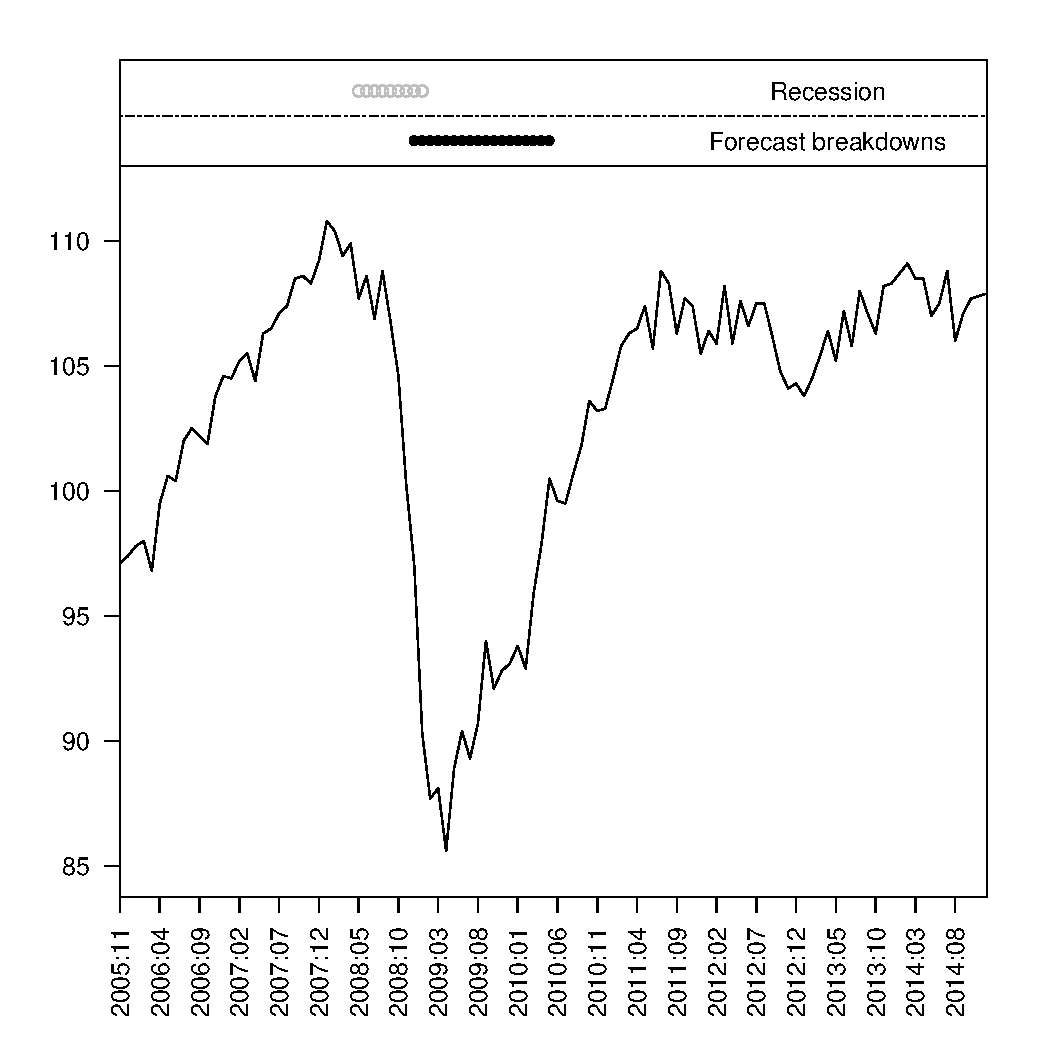
\includegraphics[scale=0.5]{H:/git/zeit-2/figs/ip_crisis_breakdowns}
\end{figure}


Large changes of the endogenous happen merely at the end of the official
recession dates and many month thereafter. At the beginning of the
official start of the recession in 2008-05 industrial production only
drops by less than 5 percent. It takes 6 more month till the end of
the ECRI dating in 2009-1 that it drops to about 80 percent of its
precrisis level. However, the trough is reached not till 2009-04.
Only in mid 2011 industrial production roughly gets back to its pre-crisis
level. 

Furthermore, most of the forecast breakdowns of single models happen
when periods at the end and long after the recession are targeted.
The instable period starts in 2008-12 and ends in 2010-06. 

\begin{figure}
\caption{Percentage of models included in MCS\label{fig:Percentage-of-models}}


\begin{centering}
\subfloat[All periods\label{fig:All-periods}]{

\centering{}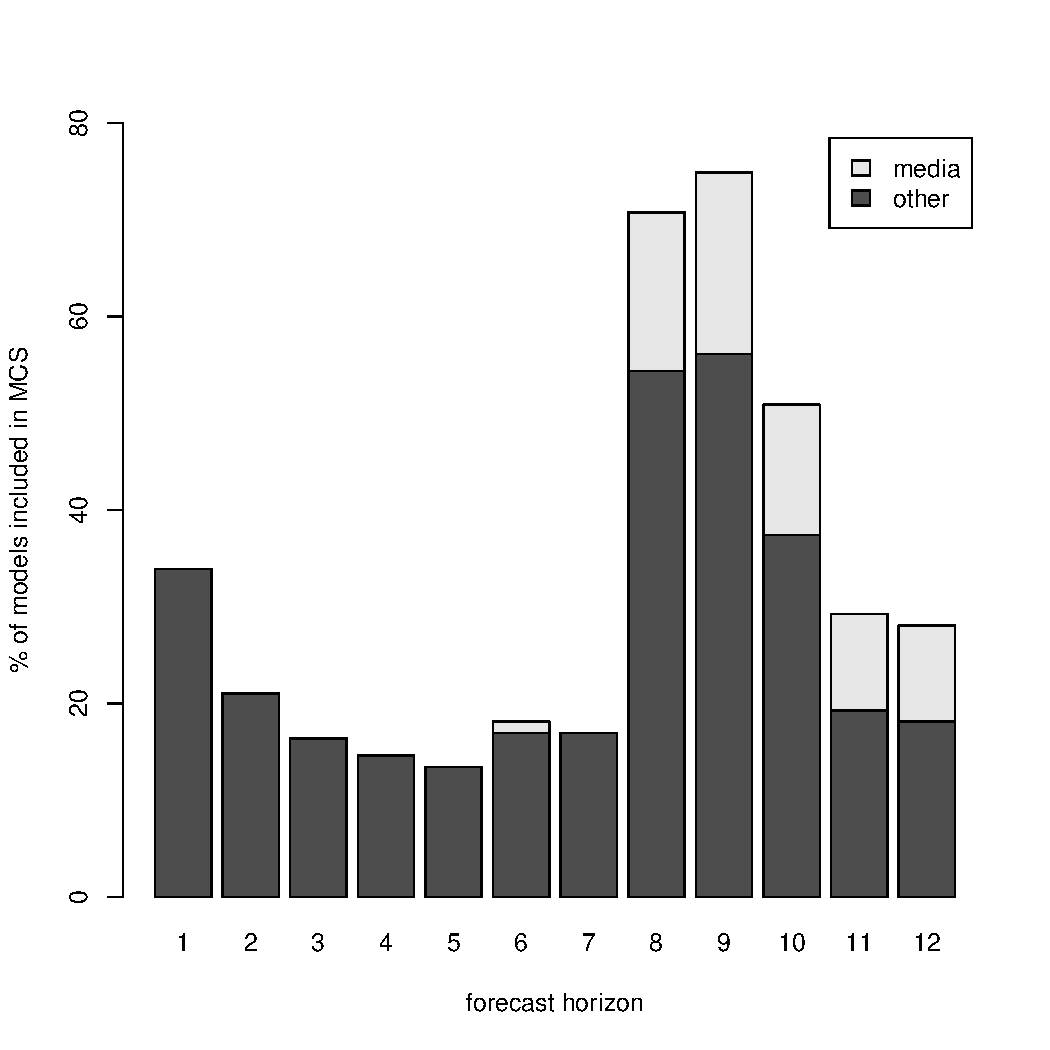
\includegraphics[scale=0.5]{H:/git/zeit-2/figs/mcs_share_media_all}}
\par\end{centering}

\centering{}\subfloat[Recession]{

\centering{}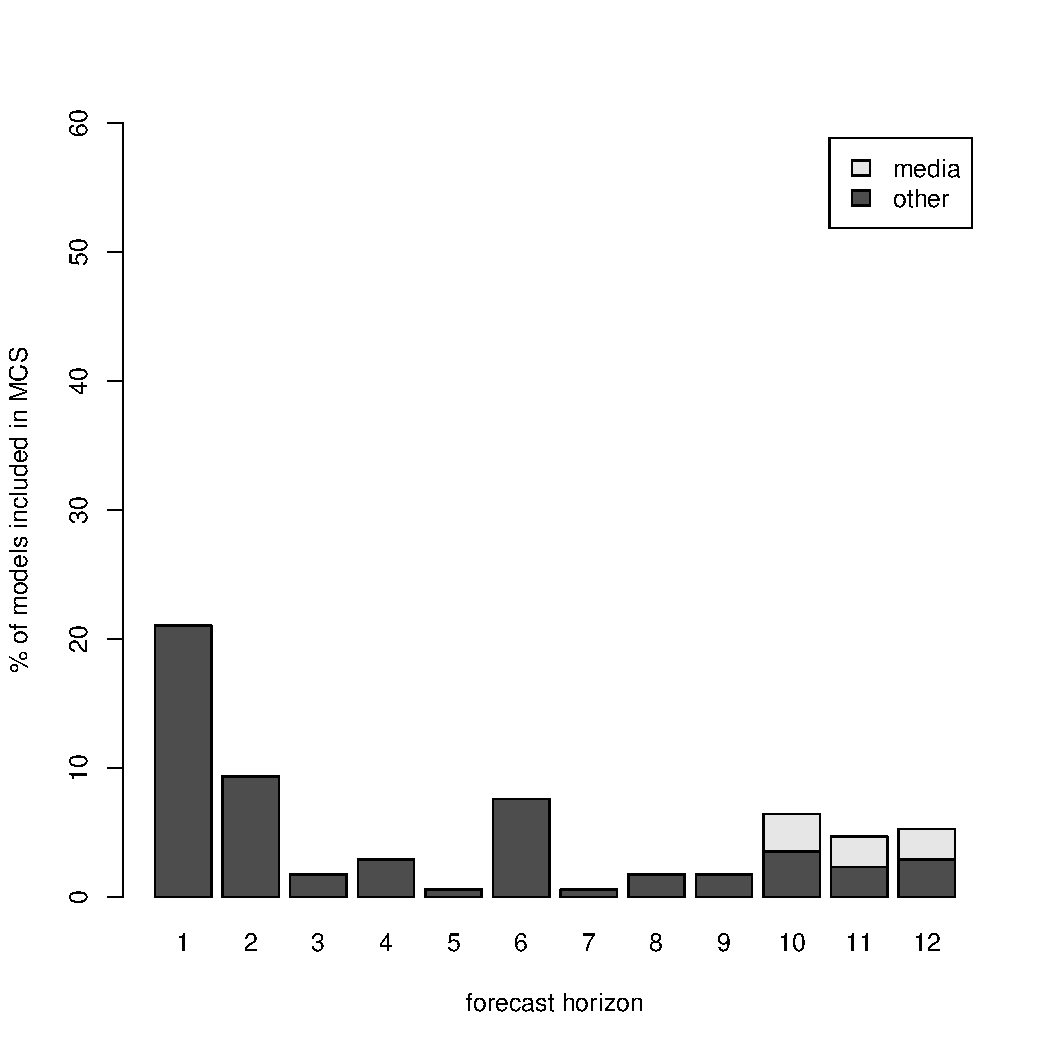
\includegraphics[scale=0.5]{H:/git/zeit-2/figs/mcs_share_media_recession}}
\end{figure}
Figure \ref{fig:Percentage-of-models} gives the percentage of media
models of the total of all models in the MCS.%
\footnote{As suggested by Hansen2011 used one size for the block bootstrapping,
6 month, and checked that the results were insensitive to different
specifications of the block size. %
} The upper panel, Panel \ref{fig:All-periods}, gives the results
over the whole range of forecasts, where each forecast horizon is
depicted individually. The differences of forecasts are relatively
informative for all horizons except the 8 and the 9 month horizon.
For all the other periods, more than 50 percent of the models are
dropped from the MCS. For short horizon up to 5 month media models
are not included in the MCS. The lower panel, Panel \ref{fig: ip, recession and forecast breakdwons},
presents the results for the instable period only. Here, the data
are very informative leading to a considerable exclusion of models
from the MCS. Media models only enter for horizons greater than 8
month.

\begin{table}
\caption{Best media models\label{tab:Best-media-models}}


\begin{centering}
\subfloat[Best media models, all periods\label{tab:Best-media-models all periods}]{\centering{}%
\begin{tabular}{c|l|c|c|c|c}
\hline 
h: & model & rmse & theilsu & rank.theilsu & \multicolumn{1}{c}{mcs.pvalue}\tabularnewline
\hline 
\hline 
1 & MT.de.present & 28.37 & 0.91 & 93 & 0.00\tabularnewline
\hline 
2 & MT.de.present & 32.73 & 0.89 & 94 & 0.00\tabularnewline
\hline 
3 & MT.present & 33.78 & 0.87 & 90 & 0.00\tabularnewline
\hline 
4 & MT.present & 31.08 & 0.84 & 71 & 0.00\tabularnewline
\hline 
5 & MT.de.present & 23.27 & 0.74 & 44 & 0.13\tabularnewline
\hline 
6 & MT.de.present & 17.50 & 0.66 & 33 & 0.25{*}\tabularnewline
\hline 
7 & MT.present & 13.33 & 0.68 & 27 & 0.24\tabularnewline
\hline 
8 & MT.present & 10.53 & 0.83{*} & 13 & 0.40{*}\tabularnewline
\hline 
9 & MT.de.future & 9.17 & 0.85{*}{*} & 5 & 0.43{*}\tabularnewline
\hline 
10 & MT.de.future & 8.43 & 0.83{*}{*} & 1 & 1.00{*}\tabularnewline
\hline 
11 & MT.de.climate & 8.69 & 0.77{*}{*} & 1 & 1.00{*}\tabularnewline
\hline 
12 & MT.de.future & 8.46 & 0.77{*}{*} & 1 & 1.00{*}\tabularnewline
\hline 
\end{tabular}}
\par\end{centering}

\begin{centering}
\subfloat[Best media models\label{tab:Best-media-models crisis}]{\centering{}%
\begin{tabular}{c|l|c|c|c|c}
\hline 
h: & model & rmse & theilsu & rank.theilsu & mcs.pvalue\tabularnewline
\hline 
\hline 
1 & MT.de.present & 63.73 & 0.88 & 92 & 0.00\tabularnewline
\hline 
2 & MT.de.present & 74.88 & 0.88 & 94 & 0.00\tabularnewline
\hline 
3 & MT.present & 77.27 & 0.85 & 89 & 0.00\tabularnewline
\hline 
4 & MT.present & 70.76 & 0.82 & 71 & 0.00\tabularnewline
\hline 
5 & MT.de.present & 51.98 & 0.72 & 46 & 0.00\tabularnewline
\hline 
6 & MT.de.present & 37.96 & 0.63 & 35 & 0.02\tabularnewline
\hline 
7 & MT.de.present & 26.60 & 0.62 & 26 & 0.00\tabularnewline
\hline 
8 & MT.present & 19.94 & 0.77 & 12 & 0.00\tabularnewline
\hline 
9 & MT.de.future & 18.09 & 0.86{*}{*} & 14 & 0.00\tabularnewline
\hline 
10 & MT.de.future & 15.90 & 0.82{*}{*} & 3 & 0.80{*}\tabularnewline
\hline 
11 & MT.de.climate & 14.08 & 0.77{*}{*} & 2 & 0.76{*}\tabularnewline
\hline 
12 & MT.de.future & 13.98 & 0.77{*}{*} & 2 & 0.89{*}\tabularnewline
\hline 
\end{tabular}}
\par\end{centering}

Note: {*} ({*}{*}) for Theil's U denotes significant outperformance
of the AR-model to the 5 (1) percent level, whereas {*} for MCS p-values
indicates, that the respective model is in the $\mathcal{M}_{75\%}^{*}$. 
\end{table}
Table \ref{tab:Best-media-models} presents the RMSE, the Theil's
U, the rank according to Theil's U and the MCS p-value of the best
media models each horizon. The upper Panel \ref{tab:Best-media-models all periods}
shows the results for all periods. Two models, MT.de.future and MT.de.climate
stick out as particularly useful for horizons from 10 to 12 months.
The former has the lowest Theil's U for 10 and 12 month horizons with
values of 0.83 and 0.77 respectively. Furthermore, for both horizons
it forms part of the $\mathcal{M}_{75\%}^{*}$ as the best model having
an MCS p-value of 1. And, it significantly outperforms the AR-model
at the 1 percent level for both horizons. For the 11 month horizon
MT.de.climate is the best model both with respect to the Theil's U
as well as the MCS p-value. It significantly outperforms the AR at
the 1 percent level, too. 

The lower Panel \ref{tab:Best-media-models crisis} shows that the
results remain robust for the instable period. MT.de.future has a
Theil's U of 0.82 and 0.77 for the 10 and 12 month horizon forecasts
and significantly outperforms the AR-model. However, it is slightly
worse according to the rank attaining only the third and second rank
for the 10 and 11 month horizon. And, while still forming part of
$\mathcal{M}_{75\%}^{*}$ having high MCS p-values of 0.80 and 0.89
for the 10 and 12 month horizon it is not the best model in the MCS.
MT.de.climate significantly outperforms the AR ranking second for
the 11 month forecast horizon. As with MT.de.future, it is not the
best model in the $\mathcal{M}_{75\%}^{*}$ having a MCS p-value of
0.76.

\begin{table}
\caption{Percentage of forecast breakdowns\label{tab:Percentage-of-forecast}}


\centering{}%
\begin{tabular}{lcccccc}
Models & \multicolumn{2}{c}{h=10} & \multicolumn{2}{c}{h=11} & \multicolumn{2}{c}{h=12}\tabularnewline
 & all periods & instable & all periods & instable & all periods & instable\tabularnewline
\hline 
\hline 
MT.de.future & 0.19 & 0.74 & 0.21 & 0.58 & 0.20 & 0.63\tabularnewline
MT.de.climate & 0.18 & 0.58 & 0.20 & 0.58 & 0.23 & 0.68\tabularnewline
mean all models & 0.19 & 0.56 & 0.20 & 0.51 & 0.21 & 0.51\tabularnewline
\hline 
\end{tabular}
\end{table}
In the first two rows Table \ref{tab:Percentage-of-forecast} shows
the percentage of times MT.de.future and MT.de.climate have failed
over all periods and the instable period for horizons 10 to 12 . The
third row shows the respective averages over all models. A value of
0 implies that the model has never failed whereas a value of 1 means
that the model has always failed. For all periods, the average of
all models rises sligthly from h=10 to h=12 from 0.19 to 0.21. Both
media models' percentage are roughly at the same level. However, for
the instable periods, they are markedly less reliable than the average.
On average all models fail 56, 51, and 51 percent of times for horizons
10, 11, and 12 respectively. MT.de.future fails in 74, 58, and 63
percent of times, whereas MT.de.climate fails in 58, 58, and 68 percent
of times for horizons 10, 11, and 12, respectively. 


\part*{Appendix}

\begin{table*}
\begin{centering}
\caption{Indicators and labels\label{tab:Indicators-and-labels}}
{\tiny{}}%
\begin{tabular}{|l|l|l|c|c|c|c|c|}
\hline 
{\tiny{}Block} & {\tiny{}Name} & {\tiny{}Label} & {\tiny{}L} & {\tiny{}D} & {\tiny{}Dln} & {\tiny{}D2ln} & {\tiny{}Lag}\tabularnewline
\hline 
\hline 
{\tiny{}Dependent variable} &  &  &  &  &  &  & \tabularnewline
\hline 
 & {\tiny{}Industrial production} & {\tiny{}IP} & {\tiny{}-} & {\tiny{}-} & {\tiny{}1} & {\tiny{}-} & {\tiny{}0}\tabularnewline
\hline 
{\tiny{}Financial } &  &  &  &  &  &  & \tabularnewline
\hline 
 & {\tiny{}Money market rate (mth.avg.)} & {\tiny{}IS-M} & {\tiny{}1} & {\tiny{}1} & {\tiny{}-} & {\tiny{}-} & {\tiny{}0}\tabularnewline
\hline 
 & {\tiny{}Discount rate/short term repo rate (mth.avg.)} & {\tiny{}IS-D} & {\tiny{}1} & {\tiny{}1} & {\tiny{}-} & {\tiny{}-} & {\tiny{}0}\tabularnewline
\hline 
 & {\tiny{}3m-money market rate (mth.avg.)} & {\tiny{}IS-3M} & {\tiny{}1} & {\tiny{}1} & {\tiny{}-} & {\tiny{}-} & {\tiny{}0}\tabularnewline
\hline 
 & {\tiny{}Yields on debt securities outstanding (mat.3-5 years)} & {\tiny{}IL-3} & {\tiny{}1} & {\tiny{}1} & {\tiny{}-} & {\tiny{}-} & {\tiny{}0}\tabularnewline
\hline 
 & {\tiny{}Yields on debt securities outstanding (mat.5-8 years)} & {\tiny{}IL-5} & {\tiny{}1} & {\tiny{}1} & {\tiny{}-} & {\tiny{}-} & {\tiny{}0}\tabularnewline
\hline 
 & {\tiny{}Long term government bond yield-9-10 years} & {\tiny{}IL-10} & {\tiny{}1} & {\tiny{}1} & {\tiny{}-} & {\tiny{}-} & {\tiny{}0}\tabularnewline
\hline 
 & {\tiny{}Term spread (10y - money market rate)} & {\tiny{}SPR-10Y-M} & {\tiny{}1} & {\tiny{}-} & {\tiny{}-} & {\tiny{}-} & {\tiny{}0}\tabularnewline
\hline 
 & {\tiny{}Term spread (10y - discount rate)} & {\tiny{}SPR-10Y-D} & {\tiny{}1} & {\tiny{}-} & {\tiny{}-} & {\tiny{}-} & {\tiny{}0}\tabularnewline
\hline 
 & {\tiny{}Term spread (10y - 3 month-money market rate)} & {\tiny{}SPR-10Y-3M} & {\tiny{}1} & {\tiny{}-} & {\tiny{}-} & {\tiny{}-} & {\tiny{}0}\tabularnewline
\hline 
 & {\tiny{}Term spread (discount rate - money market rate)} & {\tiny{}SPR-1D-M} & {\tiny{}1} & {\tiny{}-} & {\tiny{}-} & {\tiny{}-} & {\tiny{}0}\tabularnewline
\hline 
 & {\tiny{}Corporate bond-government bonds} & {\tiny{}SPR-C-G} & {\tiny{}1} & {\tiny{}-} & {\tiny{}-} & {\tiny{}-} & {\tiny{}0}\tabularnewline
\hline 
 & {\tiny{}Nomi-l effective exchange rate} & {\tiny{}EX} & {\tiny{}-} & {\tiny{}-} & {\tiny{}1} & {\tiny{}-} & {\tiny{}1}\tabularnewline
\hline 
 & {\tiny{}Real effective exchange rate} & {\tiny{}EXR} & {\tiny{}-} & {\tiny{}-} & {\tiny{}1} & {\tiny{}-} & {\tiny{}1}\tabularnewline
\hline 
 & {\tiny{}DAX} & {\tiny{}DAX} & {\tiny{}-} & {\tiny{}-} & {\tiny{}1} & {\tiny{}-} & {\tiny{}0}\tabularnewline
\hline 
 & {\tiny{}DAX vola new} & {\tiny{}VOLA1} & {\tiny{}1} & {\tiny{}1} & {\tiny{}-} & {\tiny{}-} & {\tiny{}0}\tabularnewline
\hline 
 & {\tiny{}DAX vola old} & {\tiny{}VOLA2} & {\tiny{}1} & {\tiny{}1} & {\tiny{}-} & {\tiny{}-} & {\tiny{}0}\tabularnewline
\hline 
 & {\tiny{}Hwwa index of world market prices of raw mats.} & {\tiny{}HWWA} & {\tiny{}-} & {\tiny{}-} & {\tiny{}1} & {\tiny{}1} & {\tiny{}1}\tabularnewline
\hline 
 & {\tiny{}Hwwa index, real} & {\tiny{}HWWAR} & {\tiny{}-} & {\tiny{}-} & {\tiny{}1} & {\tiny{}1} & {\tiny{}-}\tabularnewline
\hline 
 & {\tiny{}Hwwa index \textasciitilde{},energy} & {\tiny{}HWWA-E} & {\tiny{}-} & {\tiny{}-} & {\tiny{}1} & {\tiny{}1} & {\tiny{}1}\tabularnewline
\hline 
 & {\tiny{}Hwwa index, energy real} & {\tiny{}HWWA-ER} & {\tiny{}-} & {\tiny{}-} & {\tiny{}1} & {\tiny{}1} & {\tiny{}-}\tabularnewline
\hline 
 & {\tiny{}Hwwa index \textasciitilde{},excl. energy} & {\tiny{}HWWA-EX} & {\tiny{}-} & {\tiny{}-} & {\tiny{}1} & {\tiny{}1} & {\tiny{}1}\tabularnewline
\hline 
 & {\tiny{}Hwwa index, excl. energy real} & {\tiny{}HWWA-EXR} & {\tiny{}-} & {\tiny{}-} & {\tiny{}1} & {\tiny{}1} & {\tiny{}-}\tabularnewline
\hline 
 & {\tiny{}Oil prices (euros per barrel)} & {\tiny{}OIL} & {\tiny{}-} & {\tiny{}-} & {\tiny{}1} & {\tiny{}1} & {\tiny{}0}\tabularnewline
\hline 
 & {\tiny{}Oil prices (euros per barrel), real} & {\tiny{}OILR} & {\tiny{}-} & {\tiny{}-} & {\tiny{}1} & {\tiny{}1} & {\tiny{}-}\tabularnewline
\hline 
{\tiny{}Surveys} &  &  &  &  &  &  & \tabularnewline
\hline 
 & {\tiny{}Ifo index climate} & {\tiny{}IFO-C} & {\tiny{}1} & {\tiny{}1} & {\tiny{}-} & {\tiny{}-} & {\tiny{}0}\tabularnewline
\hline 
 & {\tiny{}Ifo expectations climate} & {\tiny{}IFO-EXP} & {\tiny{}1} & {\tiny{}1} & {\tiny{}-} & {\tiny{}-} & {\tiny{}0}\tabularnewline
\hline 
 & {\tiny{}Ifo index manufacturing} & {\tiny{}IFOM-C} & {\tiny{}1} & {\tiny{}1} & {\tiny{}-} & {\tiny{}-} & {\tiny{}0}\tabularnewline
\hline 
 & {\tiny{}Ifo expectations manufacturing} & {\tiny{}IFOM-EXP} & {\tiny{}1} & {\tiny{}1} & {\tiny{}-} & {\tiny{}-} & {\tiny{}0}\tabularnewline
\hline 
 & {\tiny{}Ifo index capital goods} & {\tiny{}IFOMI-C} & {\tiny{}1} & {\tiny{}1} & {\tiny{}-} & {\tiny{}-} & {\tiny{}0}\tabularnewline
\hline 
 & {\tiny{}Ifo expecations capital goods} & {\tiny{}IFOMI-EXP} & {\tiny{}1} & {\tiny{}1} & {\tiny{}-} & {\tiny{}-} & {\tiny{}0}\tabularnewline
\hline 
 & {\tiny{}Ifo index intermediate goods} & {\tiny{}IFOMV-C} & {\tiny{}1} & {\tiny{}1} & {\tiny{}-} & {\tiny{}-} & {\tiny{}0}\tabularnewline
\hline 
 & {\tiny{}Ifo expectations intermediate goods} & {\tiny{}IFOMV-EXP} & {\tiny{}1} & {\tiny{}1} & {\tiny{}-} & {\tiny{}-} & {\tiny{}0}\tabularnewline
\hline 
 & {\tiny{}Ifo index wholesale} & {\tiny{}IFOWH-C} & {\tiny{}1} & {\tiny{}1} & {\tiny{}-} & {\tiny{}-} & {\tiny{}0}\tabularnewline
\hline 
 & {\tiny{}Ifo expectations wholesale} & {\tiny{}IFOWH-EXP} & {\tiny{}1} & {\tiny{}1} & {\tiny{}-} & {\tiny{}-} & {\tiny{}0}\tabularnewline
\hline 
 & {\tiny{}GFK consumer climate survey - business cycle expectations} & {\tiny{}GFK-EXP} & {\tiny{}1} & {\tiny{}1} & {\tiny{}-} & {\tiny{}-} & {\tiny{}0}\tabularnewline
\hline 
 & {\tiny{}ZEW economic sentiment} & {\tiny{}ZEW} & {\tiny{}1} & {\tiny{}1} & {\tiny{}-} & {\tiny{}-} & {\tiny{}0}\tabularnewline
\hline 
 & {\tiny{}Assessment of order-book levels } & {\tiny{}ECBS2} & {\tiny{}1} & {\tiny{}1} & {\tiny{}-} & {\tiny{}-} & {\tiny{}0}\tabularnewline
\hline 
 & {\tiny{}Assessment of export order-book levels } & {\tiny{}ECBS3} & {\tiny{}1} & {\tiny{}1} & {\tiny{}-} & {\tiny{}-} & {\tiny{}0}\tabularnewline
\hline 
 & {\tiny{}Assessment of stocks of finished products } & {\tiny{}ECBS4} & {\tiny{}1} & {\tiny{}1} & {\tiny{}-} & {\tiny{}-} & {\tiny{}0}\tabularnewline
\hline 
 & {\tiny{}Production expectations for the months ahead } & {\tiny{}ECBS5} & {\tiny{}1} & {\tiny{}1} & {\tiny{}-} & {\tiny{}-} & {\tiny{}0}\tabularnewline
\hline 
 & {\tiny{}Selling price expectations for the months ahead } & {\tiny{}ECBS6} & {\tiny{}1} & {\tiny{}1} & {\tiny{}-} & {\tiny{}-} & {\tiny{}0}\tabularnewline
\hline 
 & {\tiny{}Employment expectations for the months ahead } & {\tiny{}ECBS7} & {\tiny{}1} & {\tiny{}1} & {\tiny{}-} & {\tiny{}-} & {\tiny{}0}\tabularnewline
\hline 
 & {\tiny{}Industrial confidence indicator (40\%)} & {\tiny{}ESI-INDU} & {\tiny{}1} & {\tiny{}1} & {\tiny{}-} & {\tiny{}-} & {\tiny{}0}\tabularnewline
\hline 
 & {\tiny{}Services confidence indicator (30\%)} & {\tiny{}ESI-SERV} & {\tiny{}1} & {\tiny{}1} & {\tiny{}-} & {\tiny{}-} & {\tiny{}0}\tabularnewline
\hline 
 & {\tiny{}Consumer confidence indicator (20\%)} & {\tiny{}ESI-C} & {\tiny{}1} & {\tiny{}1} & {\tiny{}-} & {\tiny{}-} & {\tiny{}0}\tabularnewline
\hline 
 & {\tiny{}Retail trade confidence indicator (5\%)} & {\tiny{}ESI-TRADE} & {\tiny{}1} & {\tiny{}1} & {\tiny{}-} & {\tiny{}-} & {\tiny{}0}\tabularnewline
\hline 
 & {\tiny{}Construction confidence indicator (5\%)} & {\tiny{}ESI-CTR} & {\tiny{}1} & {\tiny{}1} & {\tiny{}-} & {\tiny{}-} & {\tiny{}0}\tabularnewline
\hline 
 & {\tiny{}Economic sentiment indicator (average)} & {\tiny{}ESI} & {\tiny{}1} & {\tiny{}1} & {\tiny{}-} & {\tiny{}-} & {\tiny{}0}\tabularnewline
\hline 
 & {\tiny{}Confidence Indicator (Q2 + Q4 - Q7 + Q11) / 4 } & {\tiny{}ECCS99} & {\tiny{}1} & {\tiny{}1} & {\tiny{}-} & {\tiny{}-} & {\tiny{}0}\tabularnewline
\hline 
 & {\tiny{}Fi-ncial situation over last 12 months} & {\tiny{}ECCS1} & {\tiny{}1} & {\tiny{}1} & {\tiny{}-} & {\tiny{}-} & {\tiny{}0}\tabularnewline
\hline 
 & {\tiny{}Fi-ncial situation over next 12 months} & {\tiny{}ECCS2} & {\tiny{}1} & {\tiny{}1} & {\tiny{}-} & {\tiny{}-} & {\tiny{}0}\tabularnewline
\hline 
 & {\tiny{}General economic situation over last 12 months} & {\tiny{}ECCS3} & {\tiny{}1} & {\tiny{}1} & {\tiny{}-} & {\tiny{}-} & {\tiny{}0}\tabularnewline
\hline 
 & {\tiny{}General economic situation over next 12 months} & {\tiny{}ECCS4} & {\tiny{}1} & {\tiny{}1} & {\tiny{}-} & {\tiny{}-} & {\tiny{}0}\tabularnewline
\hline 
 & {\tiny{}Price trends over last 12 months} & {\tiny{}ECCS5} & {\tiny{}1} & {\tiny{}1} & {\tiny{}-} & {\tiny{}-} & {\tiny{}0}\tabularnewline
\hline 
 & {\tiny{}Price trends over next 12 months} & {\tiny{}ECCS6} & {\tiny{}1} & {\tiny{}1} & {\tiny{}-} & {\tiny{}-} & {\tiny{}0}\tabularnewline
\hline 
 & {\tiny{}Unemployment expectations over next 12 months} & {\tiny{}ECCS7} & {\tiny{}1} & {\tiny{}1} & {\tiny{}-} & {\tiny{}-} & {\tiny{}0}\tabularnewline
\hline 
 & {\tiny{}Major purchases at present} & {\tiny{}ECCS8} & {\tiny{}1} & {\tiny{}1} & {\tiny{}-} & {\tiny{}-} & {\tiny{}0}\tabularnewline
\hline 
 & {\tiny{}Major purchases over next 12 months} & {\tiny{}ECCS9} & {\tiny{}1} & {\tiny{}1} & {\tiny{}-} & {\tiny{}-} & {\tiny{}0}\tabularnewline
\hline 
 & {\tiny{}Savings at present} & {\tiny{}ECCS10} & {\tiny{}1} & {\tiny{}1} & {\tiny{}-} & {\tiny{}-} & {\tiny{}0}\tabularnewline
\hline 
 & {\tiny{}Savings over next 12 months} & {\tiny{}ECCS11} & {\tiny{}1} & {\tiny{}1} & {\tiny{}-} & {\tiny{}-} & {\tiny{}0}\tabularnewline
\hline 
 & {\tiny{}Statement on fi-ncial situation of household} & {\tiny{}ECCS12} & {\tiny{}1} & {\tiny{}1} & {\tiny{}-} & {\tiny{}-} & {\tiny{}0}\tabularnewline
\hline 
{\tiny{}Prices and wages} &  &  &  &  &  &  & \tabularnewline
\hline 
 & {\tiny{}CPI} & {\tiny{}CPI} & {\tiny{}-} & {\tiny{}-} & {\tiny{}1} & {\tiny{}1} & {\tiny{}0}\tabularnewline
\hline 
 & {\tiny{}Core CPI} & {\tiny{}CPI-EX} & {\tiny{}-} & {\tiny{}-} & {\tiny{}1} & {\tiny{}1} & {\tiny{}0}\tabularnewline
\hline 
 & {\tiny{}Negotiated wage and salary level} & {\tiny{}TARIF} & {\tiny{}-} & {\tiny{}-} & {\tiny{}1} & {\tiny{}1} & {\tiny{}0}\tabularnewline
\hline 
{\tiny{}Real economy} &  &  &  &  &  &  & \tabularnewline
\hline 
 & {\tiny{}Intermediate goods production} & {\tiny{}IP-VORL} & {\tiny{}-} & {\tiny{}-} & {\tiny{}1} & {\tiny{}-} & {\tiny{}0}\tabularnewline
\hline 
 & {\tiny{}Manufacturing orders - consumer goods} & {\tiny{}ORD-C} & {\tiny{}-} & {\tiny{}-} & {\tiny{}1} & {\tiny{}-} & {\tiny{}0}\tabularnewline
\hline 
 & {\tiny{}Manufacturing orders - capital goods} & {\tiny{}ORD-I} & {\tiny{}-} & {\tiny{}-} & {\tiny{}1} & {\tiny{}-} & {\tiny{}0}\tabularnewline
\hline 
 & {\tiny{}Employed persons (work-place concept)} & {\tiny{}EW} & {\tiny{}-} & {\tiny{}-} & {\tiny{}1} & {\tiny{}-} & {\tiny{}0}\tabularnewline
\hline 
 & {\tiny{}1+unemployment (\% civilian labour)} & {\tiny{}ALQ} & {\tiny{}-} & {\tiny{}1} & {\tiny{}-} & {\tiny{}-} & {\tiny{}1}\tabularnewline
\hline 
 & {\tiny{}Vacancies} & {\tiny{}VAC} & {\tiny{}-} & {\tiny{}-} & {\tiny{}1} & {\tiny{}-} & {\tiny{}1}\tabularnewline
\hline 
 & {\tiny{}Capacity utilisation} & {\tiny{}CAPA} & {\tiny{}1} & {\tiny{}1} & {\tiny{}-} & {\tiny{}-} & {\tiny{}0}\tabularnewline
\hline 
 & {\tiny{}Hours worked} & {\tiny{}WHOUR} & {\tiny{}1} & {\tiny{}1} & {\tiny{}-} & {\tiny{}-} & {\tiny{}0}\tabularnewline
\hline 
{\tiny{}Composite indicators} &  &  &  &  &  &  & \tabularnewline
\hline 
 & {\tiny{}FAZ indicator} & {\tiny{}FAZ} & {\tiny{}-} & {\tiny{}-} & {\tiny{}1} & {\tiny{}-} & {\tiny{}1}\tabularnewline
\hline 
 & {\tiny{}Composite leading indicator (amplitude restored)} & {\tiny{}OECDL1} & {\tiny{}1} & {\tiny{}1} & {\tiny{}-} & {\tiny{}-} & {\tiny{}2}\tabularnewline
\hline 
 & {\tiny{}Composite leading indicator (trend restored)} & {\tiny{}OECDL2} & {\tiny{}-} & {\tiny{}1} & {\tiny{}-} & {\tiny{}-} & {\tiny{}2}\tabularnewline
\hline 
 & {\tiny{}Composite leading indicator (normalized)} & {\tiny{}OECDL3} & {\tiny{}1} & {\tiny{}1} & {\tiny{}-} & {\tiny{}-} & {\tiny{}2}\tabularnewline
\hline 
{\tiny{}Media indicators} &  &  &  &  &  &  & \tabularnewline
\hline 
 & {\tiny{}all observations} & {\tiny{}MT.all} & {\tiny{}1} & {\tiny{}1} & {\tiny{}-} & {\tiny{}-} & {\tiny{}0}\tabularnewline
\hline 
 & {\tiny{}all observations related to the future} & {\tiny{}MT.future} & {\tiny{}1} & {\tiny{}1} & {\tiny{}-} & {\tiny{}-} & {\tiny{}0}\tabularnewline
\hline 
 & {\tiny{}all observations related to the present} & {\tiny{}MT.presence} & {\tiny{}1} & {\tiny{}1} & {\tiny{}-} & {\tiny{}-} & {\tiny{}0}\tabularnewline
\hline 
 & {\tiny{}all observations related to the future and present} & {\tiny{}MT.climate} & {\tiny{}1} & {\tiny{}1} & {\tiny{}-} & {\tiny{}-} & {\tiny{}0}\tabularnewline
\hline 
 & {\tiny{}all observations related to Germany} & {\tiny{}MT.de} & {\tiny{}1} & {\tiny{}1} & {\tiny{}-} & {\tiny{}-} & {\tiny{}0}\tabularnewline
\hline 
 & {\tiny{}All observations related to Germany and the future} & {\tiny{}MT.de.future} & {\tiny{}1} & {\tiny{}1} & {\tiny{}-} & {\tiny{}-} & {\tiny{}0}\tabularnewline
\hline 
 & {\tiny{}All observations related to Germany and present} & {\tiny{}MT.de.present} & {\tiny{}1} & {\tiny{}1} & {\tiny{}-} & {\tiny{}-} & {\tiny{}0}\tabularnewline
\hline 
 & {\tiny{}All observations related to Germany, and future and present} & {\tiny{}MT.de.climate} & {\tiny{}1} & {\tiny{}1} & {\tiny{}-} & {\tiny{}-} & {\tiny{}0}\tabularnewline
\hline 
 & {\tiny{}All observations related to government budget} & {\tiny{}MT.budget} & {\tiny{}1} & {\tiny{}1} & {\tiny{}-} & {\tiny{}-} & {\tiny{}0}\tabularnewline
\hline 
 & {\tiny{}All observations related to monetary issues} & {\tiny{}MT.currency} & {\tiny{}1} & {\tiny{}1} & {\tiny{}-} & {\tiny{}-} & {\tiny{}0}\tabularnewline
\hline 
 & {\tiny{}All observations related to the labor market} & {\tiny{}MT.labor} & {\tiny{}1} & {\tiny{}1} & {\tiny{}-} & {\tiny{}-} & {\tiny{}0}\tabularnewline
\hline 
 & {\tiny{}All observations related to the business cycle} & {\tiny{}MT.cycle} & {\tiny{}1} & {\tiny{}1} & {\tiny{}-} & {\tiny{}-} & {\tiny{}0}\tabularnewline
\hline 
 & {\tiny{}All observations related to taxation} & {\tiny{}MT.taxation} & {\tiny{}1} & {\tiny{}1} & {\tiny{}-} & {\tiny{}-} & {\tiny{}0}\tabularnewline
\hline 
 & {\tiny{}All observations related to the German government budget} & {\tiny{}MT.de.budget} & {\tiny{}1} & {\tiny{}1} & {\tiny{}-} & {\tiny{}-} & {\tiny{}0}\tabularnewline
\hline 
 & {\tiny{}All observations related to the German labor market} & {\tiny{}MT.de.labor} & {\tiny{}1} & {\tiny{}1} & {\tiny{}-} & {\tiny{}-} & {\tiny{}0}\tabularnewline
\hline 
 & {\tiny{}All observations related to the German business cycle} & {\tiny{}MT.de.cycle} & {\tiny{}1} & {\tiny{}1} & {\tiny{}-} & {\tiny{}-} & {\tiny{}0}\tabularnewline
\hline 
 & {\tiny{}All observations related to German taxation} & {\tiny{}MT.de.taxation} & {\tiny{}1} & {\tiny{}1} & {\tiny{}-} & {\tiny{}-} & {\tiny{}0}\tabularnewline
\hline 
\end{tabular}
\par\end{centering}{\tiny \par}

\end{table*}


\bibliographystyle{plainnat}
\bibliography{mti_ip}

\end{document}
